\documentclass{VUMIFInfKursinis}
\usepackage{algorithmicx}
\usepackage{algorithm}
\usepackage{algpseudocode}
\usepackage{amsfonts}
\usepackage{amsmath}
\usepackage{bm}
\usepackage{color}
\usepackage{graphicx}
\usepackage{hyperref}
\usepackage{url}


% Titulinio aprašas
\university{Vilniaus universitetas}
\faculty{Matematikos ir informatikos fakultetas}
\institute{Informatikos institutas}
\department{Informatikos katedra}
\papertype{0-as Namų Darbas}
\title{Trumpiausio bendro superžodžio problemos algoritmo analizė}
\titleineng{Shortest common superstring problem algorithm analysis}
\status{3 kurso 2 grupės studentas}
\author{Ričardas Čubukinas}
\supervisor{Asist., Dr. Valdas Dičiūnas}


\date{Vilnius \\ \the\year}

% Nustatymai
\setmainfont{Palem}[
  Extension = .ttf,
  Path = Palemonas/,
  UprightFont = *-nm,
  BoldFont  = *-bd , 
  ItalicFont  = *-it ,
  BoldItalicFont = *-bi ]

\bibliography{bibliografija} 



\begin{document}
\maketitle

\tableofcontents

\sectionnonum{Įvadas}
Šiame darbe nagrinėsime „Shortest Common Substring“ problemą.
\begin{itemize}
  \item{\textbf{Duota:} Baigtinė abecelė $\Sigma$, baigtinis žodžių rinkinys $R$ sudaryta iš $\Sigma{}^*$.}
  \item{\textbf{Tikslas:} Surasti trumpiausią bendrą super-žodį $\omega$, tokį kad kiekvienas rinkinio žodis $x \in R$ yra žodžio $\omega$ subžodis, pvz $\omega =\omega{}_0x\omega{}_1$, kur $\omega{}_0,\omega{}_1 \in \Sigma{}^*$.}
\end{itemize}
\cite{ausiello1999complexity}

\section{Brutalios Jėgos Algoritmas}
Tarkime turime žodžių rinkinį $R=\{AAA, ABA, AAB\}$. Paieška vykdysime brutalios jėgos algoritmu. Tikriname rinkinio $R$ išdėstymą $P_i \in P$, kur P yra visi skirtingi rinkinio išdėstymai $n!$. Kiekviename išdėstyme tikriname visus šalia esančius žodžius kiek jie persipina tarpusavyje, išsaugome maksimalų persipinimą, jei daugiau nei nulis ir pridedame persipinančius žodžius prie trumpiausio subžodžio, taip pereiname visus žodžius kol gauname tos kombinacijos trumpiausia superžodį, jį išsaugome ir taip einame per kiekvieną kombinaciją ir gautą superžodį lyginame su praeitu išsaugodami trumpesnį kol pereiname visas rinkinių kombinacijas. Pavyzdžiui:\\

\sectionnonum{Išvados}
Išvadose ir pasiūlymuose, nekartojant atskirų dalių apibendrinimų,
suformuluojamos svarbiausios darbo išvados, rekomendacijos bei pasiūlymai.

\printbibliography[heading=bibintoc] % Literatūros šaltiniai aprašomi
% bibliografija.bib faile. Šaltinių sąraše nurodoma panaudota literatūra,
% kitokie šaltiniai. Abėcėlės tvarka išdėstoma tik darbe panaudotų (cituotų,
% perfrazuotų ar bent paminėtų) mokslo leidinių, kitokių publikacijų
% bibliografiniai aprašai (šiuo punktu pasirūpina LaTeX). Aprašai pateikiami
% netransliteruoti.

%\appendix  % Priedai
%
%% Prieduose gali būti pateikiama pagalbinė, ypač darbo autoriaus savarankiškai
%% parengta, medžiaga. Savarankiški priedai gali būti pateikiami kompiuterio
%% diskelyje ar kompaktiniame diske. Priedai taip pat vadinami ir numeruojami.
%% Tekstas su priedais siejamas nuorodomis (pvz.: \ref{img:mlp}).
%
%\section{Niauroninio tinklo struktūra}
%\begin{figure}[H]
%    \centering
%    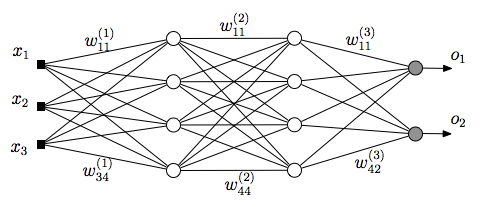
\includegraphics[scale=0.5]{img/MLP}
%    \caption{Paveikslėlio pavyzdys}   % Antraštė įterpiama po paveikslėlio
%    \label{img:mlp}
%\end{figure}
%
%% Idėti po pirmo priedo.
%\pagenumbering{gobble}
%
%\section{Eksperimentinio palyginimo rezultatai}
%% tablesgenerator.com - converts calculators (e.g. excel) tables to LaTeX
%\begin{table}[H]\footnotesize
%  \centering
%  \caption{Lentelės pavyzdys}    % Antraštė įterpiama prieš lentelę
%  {\begin{tabular}{|l|c|c|} \hline
%    Algoritmas & $\bar{x}$ & $\sigma^{2}$ \\
%    \hline
%    Algoritmas A  & 1.6335    & 0.5584       \\
%    Algoritmas B  & 1.7395    & 0.5647       \\
%    \hline
%  \end{tabular}}
%  \label{tab:table example}
%\end{table}

\end{document}
